\documentclass[UTF8]{article}
\usepackage{bm}
\usepackage{amsmath}
\usepackage{cases}
\usepackage{cite}
\usepackage{graphicx}
\usepackage[margin=1in]{geometry}
\geometry{a4paper}
\usepackage{fancyhdr}
\usepackage{array}
\pagestyle{fancy}
\usepackage{wrapfig}
\fancyhf{}
\usepackage{float}  %设置图片浮动位置的宏包
\usepackage{subfigure}
\usepackage{caption}
\usepackage{booktabs}
\usepackage{listings}
\usepackage{xcolor}
\usepackage{multirow}
\lstset{numbers=left, %设置行号位置
	numberstyle=\tiny, %设置行号大小
	keywordstyle=\color{blue}, %设置关键字颜色
	commentstyle=\color[cmyk]{1,0,1,0}, %设置注释颜色
	frame=single, %设置边框格式
	escapeinside=``, %逃逸字符(1左面的键),用于显示中文
	breaklines, %自动折行
	extendedchars=false, %解决代码跨页时,章节标题,页眉等汉字不显示的问题
	xleftmargin=2em,xrightmargin=2em, aboveskip=1em, %设置边距
	tabsize=4, %设置tab空格数
	showspaces=false %不显示空格
}

\title{The Holographic Imaging Technology}
\author{by 22 Artificial Intelligence ChenxuZhang}
\date{2023.11.01}
\pagenumbering{arabic}

\begin{document}
	
	\fancyhead[L]{ChenxuZhang}
	\fancyhead[R]{ID 202264691028}
	\fancyfoot[C]{\thepage}
	
	\maketitle
	\tableofcontents
	\newpage
	
	\section{Abstract}
British scientist Dennis Garber proposed holographic technology in 1948 to improve the resolution of electron microscope on the basis of the research of Bragg and Transnick. Holographic technology is the use of light interference and diffraction principles, the object emitted by the specific light waves in the form of interference fringes recorded, and under certain conditions to make it reproduced, the formation of realistic three-dimensional image of the technology. This technique records all the information (amplitude and phase) of the object, and is therefore also known as holography. Since it was not easy to obtain coherent light at that time, holography was not developed for ten years after its introduction. Until the introduction of the laser, 19624 Leith and others use the laser as a light source, and the use of off-axis method to successfully obtain three-dimensional images of holograms, holographic technology has been rapidly changing. 1971 Gaber for the invention of holography won the Nobel Prize in Physics. In recent years, holographic technology has been developing rapidly, from information storage, processing to remote sensing technology and industrial product testing, measurement technology and medicine and other fields are widely used, has become a new field of science and technology.
 
	
\section{Purpose of the experiment}
   $\bm{A}$.Understand the basic principles and characteristics of holography.\\
   $\bm{B}$.Preliminary mastery of the basic techniques of taking static holographic photographs and the methods of object image reproduction.

	\section{Experimental apparatus}
    Optical stage, HeNe laser, beam splitter, beam expander, reflector, subject, holographic dry plate.
    
	\begin{figure}[H]
	    	\centering
	    	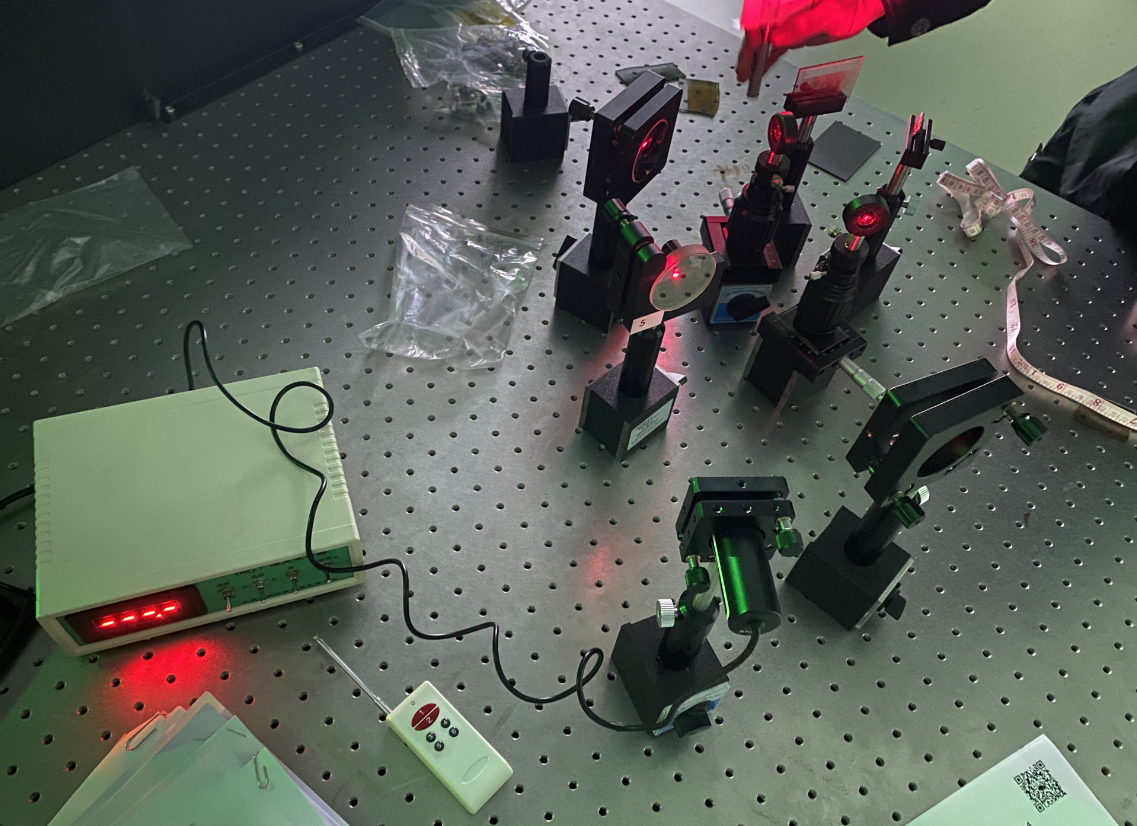
\includegraphics[clip,scale=0.6,trim={0 0 0 0}]{fig/fig1.png}
	        \caption{Related equipment display}
	        \label{figure.1}
    \end{figure}    
    
   \begin{itemize}
     \item \textbf{Optical stage}: An optical stage is a platform used to support and adjust optical components. It is typically made of sturdy materials to ensure precise optical experiments and component alignment. It often includes fine adjustment mechanisms for accurate positioning of various optical elements.
   
     \item \textbf{HeNe laser (Helium-Neon laser)}: The Helium-Neon laser is a gas laser commonly used in optical experiments and measurements. It emits visible light with a wavelength typically at 632.8 nanometers, providing a stable laser light source.
   
     \item \textbf{Beam splitter}: A beam splitter is an optical element used to split an incident light beam into two or more beams. It reflects a portion of the light while transmitting the remainder, commonly used in interferometers and optical path distribution.
   
     \item \textbf{Beam expander}: A beam expander is an optical element used to expand or reduce the diameter of a light beam. It is typically composed of lenses to change the size of the beam.
   
     \item \textbf{Reflector}: A reflector is an optical element used to change the direction of a light path. It can be a flat mirror, a reflecting prism, or a curved mirror used to reflect the light beam in the desired direction.
   
     \item \textbf{Subject}: The subject is the object or scene to be photographed or observed in optical experiments or photography.
   
     \item \textbf{Holographic dry plate}: A holographic dry plate is a photosensitive material used to record holographic images. It is typically a glass or plastic plate used to record both the phase and amplitude information of light to create holographic images.
   \end{itemize}
   
    
        
	\section{Experimental principles}  
	
	Holography is fundamentally different from ordinary photography. Ordinary photography is based on the principle of geometric optics to the object light intensity (amplitude) and wavelength (colour photography) photographed, on the negative and the object similar to the graphics. Hologram is based on fluctuating optical principles (interference and diffraction) at the same time the amplitude and phase of the object light photographed (holographic recording), on the negative to get complex interference fringes. When observing holograms, the image of the object must be diffracted by laser irradiation. Therefore, holography is divided into two processes: holographic recording and image reproduction.
	 
    \subsection{Holographic records}
    \subsubsection{Holographic recording process}
    According to the principle of light interference, monochromatic light source s through the beam splitter plate $BS$ into two beams of coherent light, one for the reference beam $r$, the other for the object beam $o$, the object light $o$ light on the object to be photographed for the reflection of the object light wave. The object light wave and the reference light wave are superimposed on the photographic substrate and interfere, forming light and dark interference fringes. The light and dark contrast of the stripes records the amplitude distribution of the object light, while the shape, spacing and position of the stripes (geometric features) records the phase distribution of the object. In radio terms, that is, through the object light wave and the object light wave modulation of the reference light wave, the photographic film will be the object light wave of all the information recorded, after the development, fixing process to obtain and diffraction grating similar to the rest of the film.
    \begin{figure}[H]
              \begin{minipage}[t]{0.5\linewidth}
                 \centering
                 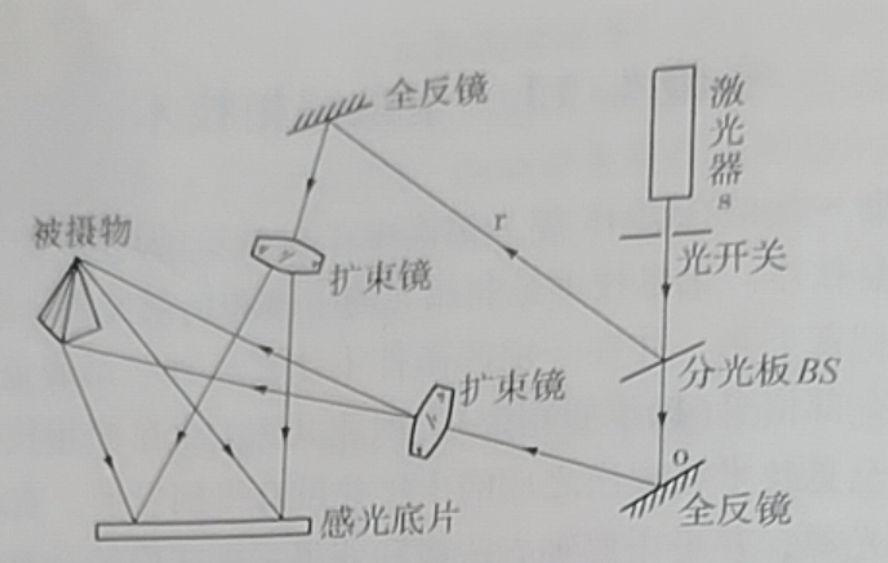
\includegraphics[clip,scale=0.51,trim={0 0 0 0}]{fig/fig2.png}
                 \label{figure.11}
                 \caption{Holographic recording process}
              \end{minipage}
              \begin{minipage}[t]{0.5\linewidth}
                 \centering
                 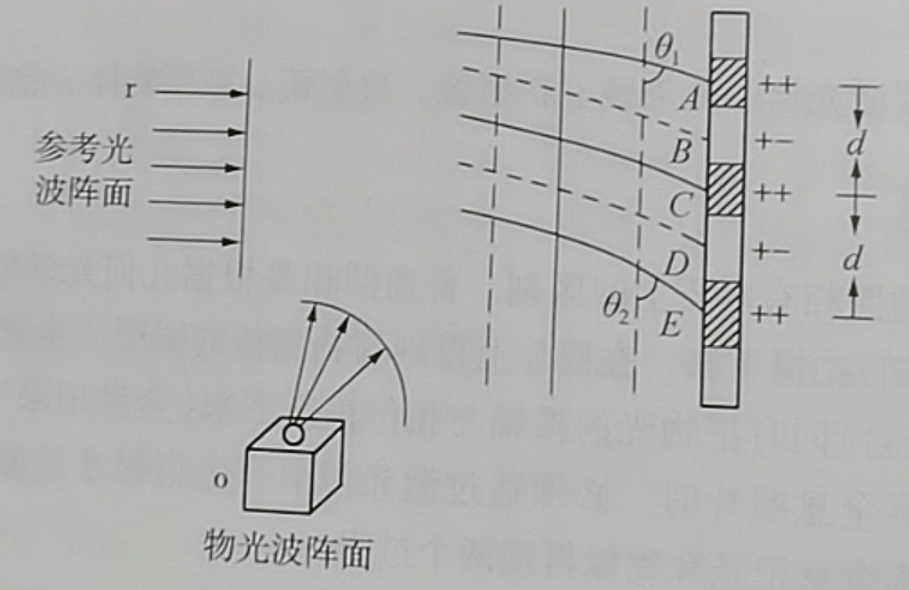
\includegraphics[clip,scale=0.49,trim={0 0 0 0}]{fig/fig3.png}
                 \label{figure.12}
                 \caption{Principle of holography reference chart}
              \end{minipage}   	  
           \end{figure}  
           
    \subsubsection{Principle of holography}
    As shown in the figure, let the reference light $r$ is a plane wave. Take the object of a light-emitting (scattered light) point o, which emits light in space to the spherical wave propagation, and the reference light for each other as coherent light. In order to simplify the discussion, the holographic negative parallel reference light $r$ wavefront, the solid line in the figure represents the wave peak, the dotted line represents the wave valley, the two wavefront can be superimposed in space, where the reference light $r$ and the object light o of the two wavefront angle $\theta$ in the negative from $A$ to $E$ is a change in the $\theta_1> \theta_2$, $\theta$ for the object light propagation direction and the reference light propagation direction of the angle, and the change also reflects the phase change of object light $o$. The holographic negative is a reference light, the reference light propagation direction of the reference light, the reference light is a reference light, the reference light is a reference light.
    
    As can be seen from the graphical method, in the negative $A, C, E$, the same phase (two peaks meet) to form interference bright lines,$ D, B $and other places in the opposite phase (peaks and valleys meet) to form dark lines. As can be seen from the figure, due to changes in $\theta$, the interference fringe spacing d on the hologram from A to E is also changing, and $d_1 < d_2$, that is, the angle $\theta$ is large, the spacing $d$ is small. Therefore, the phase change of the object light $o$ is recorded on the holographic film with the help of the change of the stripe spacing $d$. In addition, the light and dark stripes change from $A$ to $E$.
    
    In addition, the contrast between the light intensity of the dark and light stripes (stripe contrast) records the intensity of the object light $\theta$. Thus, the interference fringes of different densities and contrasts on the negative record "all the information" of the object light $o$. Similarly, for another film, the interference fringes of different densities and contrasts record the intensity of the object light $\theta$. Similarly, for another object light point P on the negative also recorded another set of different density, different contrast interference fringes. It can be assumed that the original object is made up of many points, then the holographic negative records a superposition of the interference fringes of the whole object.
    
   \subsection{Reproduction of holograms}
   The holographic negative records not an image of the subject, but complex interference fringes, which must be reproduced by certain means when observing the photograph.
   
   \subsubsection{Image reproduction process}
   The use of light wave diffraction principle, with a reference beam of light irradiation holographic film, the sparse and dense interference fringes on the negative is equivalent to a special grating (the grating constant changes reflect the phase information of the object light), the reference beam to the grating will produce diffraction, it is the first level of diffraction of light waves will be the original object light wave wave front reproduced. Therefore, we can see the stereoscopic image of the original object through the hologram. Observation, from the back of the holographic negative (receiving transmitted light) can be seen in the original position and the original object has an identical stereoscopic virtual image $O'$, while in the holographic negative symmetry of the other side of the screen has a conjugate real image $O''$.
   
   	\begin{figure}[H]
       	    	\centering
       	    	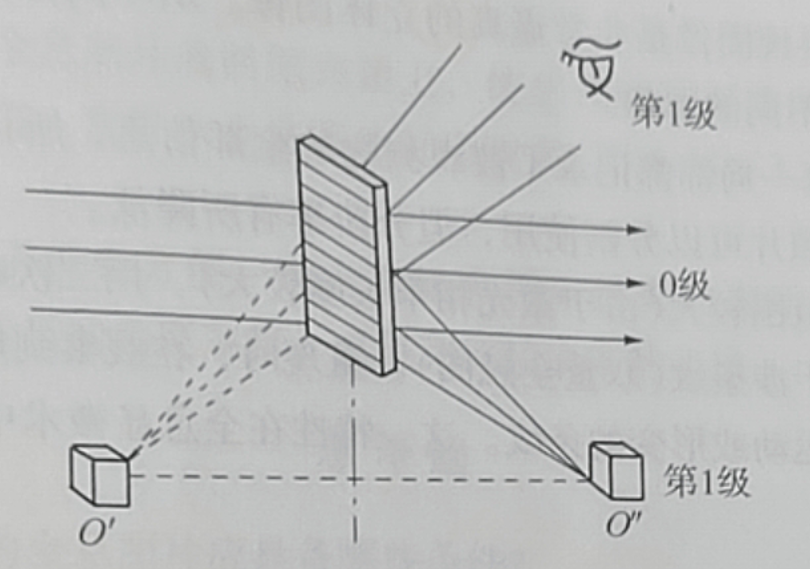
\includegraphics[clip,scale=0.6,trim={0 0 0 0}]{fig/fig4.png}
       	        \caption{Image reproduction process}
       	        \label{figure.14}
           \end{figure}    
   
   \subsubsection{Wavefront reproduction and diffraction of light}
   The regularity of the wavefront reproduction (object image) described above can be explained by the principle of diffraction of light. Holographic film interference fringes, equivalent to a special (constant change) of the grating, and therefore can be used to analyse the grating equation to discuss. In order to facilitate the analysis, set any object point element in the holographic film on the corresponding set of interference fringes (grating).
   
   grating function:
   \begin{eqnarray}
   d \sin\theta = n\lambda \qquad (n = 0,\pm 1, \pm 2,\cdots)
   \end{eqnarray}
   where $\theta$ is the diffraction angle.
   When $n = 0, \theta = 0$ is the zero-level diffracted wave. This is the attenuated wave train propagating in the direction of the reference light.
   
   When $n=1$, since $d_1<d_2$, then the diffraction angle $\theta_1> \theta_2$. From the figure, we can see that all the $n=1$ diffracted beams passing through the holographic negative are dispersed, and their prolongation line intersects at $o'$ to form an imaginary image, which is exactly the same as the original object $O$. This is the reproduction of the holographic image of the original object $O$ point.
   When n=-1, from the figure, all the diffracted beams of n=-1 level are converged, and the convergence point is the real image $o"$ of point $0'$.
   
   The original object is composed of many point elements. According to the principle of superposition of waves, the holographic film records the "holography" of all the point elements of the object, and the image of the subject is the sum of the images of these individual point elements. Therefore, we can observe a three-dimensional image of the object on the holographic film.
      	\begin{figure}[H]
          	    	\centering
          	    	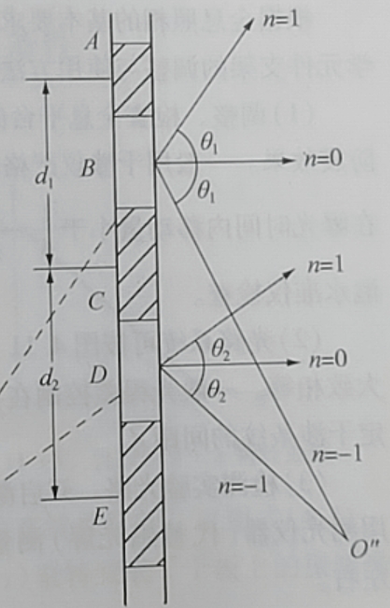
\includegraphics[clip,scale=0.8,trim={0 0 0 0}]{fig/fig5.png}
          	        \caption{Wavefront reproduction and diffraction of light}
          	        \label{figure.14}
              \end{figure}
   
               
	\section{Contents and Steps}
    \subsubsection{Modulated hologram optical path system}
    According to the basic requirements of holography, in the application of holography should first understand, familiar with the holography of the experimental equipment, instruments and optical components of the adjustment and use of the support.
    
    \begin{itemize}
      \item Adjust and inspect the levelness and stability of the holographic platform. In this experiment, an optical platform setup is employed to achieve good vibration damping. Use an interferometer for a thorough check or assemble a Michelson interferometer on the holographic table. If the interference fringes move less than one-fourth to one-half fringe spacing during the exposure time, the basic experimental conditions are met. The platform's levelness can be checked using a bubble level.
    
      \item Arrange the optical components in the optical path system as shown in the diagram, ensuring that the centers of all optical elements are at the same height, and the optical path lengths for the object light and reference light are roughly equal. Typically, keep the optical path difference within 2 cm. The angle θ between the object light and the reference light should be in the range of 30° to 45°, which determines the spacing of interference fringes, denoted as 'd'.
    
      \item Verify the experimental optical path. Turn on the laser power supply and adjust the beam expander and reflector to evenly illuminate the photosensitive plate with object light and reference light. Measure the relative intensity of the object light and reference light (i.e., the beam splitter ratio) using a photometric instrument (in place of the photosensitive plate). Aim for a ratio of approximately 3:5.
    \end{itemize}
    
       	\begin{figure}[H]
           	    	\centering
           	    	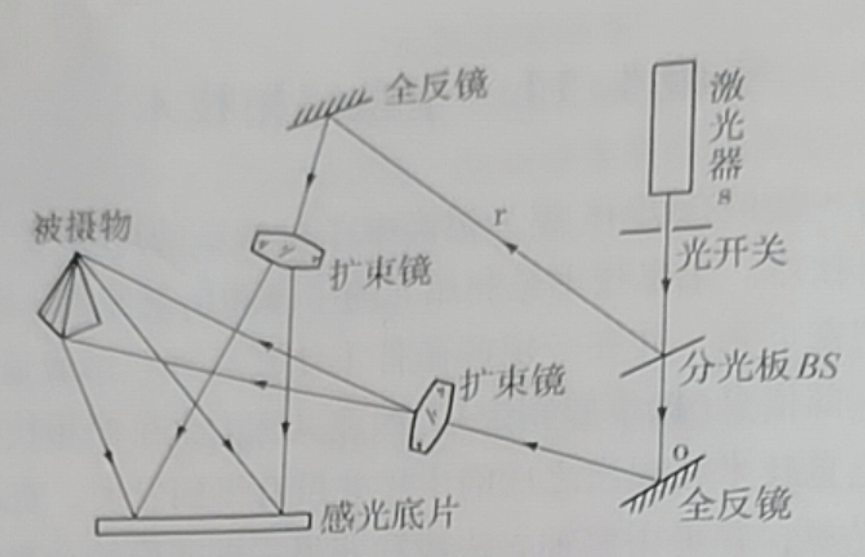
\includegraphics[clip,scale=1,trim={0 0 0 0}]{fig/fig6.png}
           	        \caption{Modulated hologram optical path system reference chart }
           	        \label{figure.14}
               \end{figure}
    
    \subsubsection{Taking static holograms}
    \begin{itemize}
      \item Determine the exposure time based on the properties of the photosensitive plate, including the resolution of the photosensitive material and the sensitivity of the plate, as well as the intensity of the light source. Typically, an exposure time of $8 to 10$ seconds is selected. It is advisable to determine the optimal exposure time through test exposures before adjusting the exposure timer further.
    
      \item Turn off the laser power supply and, in a darkroom, place the photosensitive plate on a plate holder. Ensure that the emulsion side (film emulsion) faces the object to receive the object light.
    
      \item Wait for a few minutes before turning on the laser power for exposure. During the exposure process, it is strictly forbidden to touch the vibration isolation table and any optical components.
    
      \item After the exposure is complete, remove the photosensitive plate for processing. The developing and fixing processes are similar to regular photographic film. Typically, development takes $20 to 30$ seconds, and fixing requires $5 to 10$ minutes. In the experiment, you can consider the plate turning gray under green light as an indicator for the right time to remove the plate, which often results in better outcomes. To enhance the diffraction capability of the hologram, you can bleach the plate after fixing.
    \end{itemize}
    
    \subsubsection{Observation of reproduced object images from holograms}
    \begin{itemize}
      \item Observe virtual images: Place the hologram back into its original holder, ensuring that the photosensitive emulsion side faces the reference light (the laser beam received by the beam expander). Initially, block the object light beam and observe directly from the back of the hologram. This allows you to see virtual images at the original object positions.
    
      \item Observe real images: For convenience in observation, it is common to use the unexpanded laser beam shining on the reverse side of the hologram (the non-photosensitive emulsion side). By selecting an appropriate angle for observation, you can obtain relatively clear real images.
    \end{itemize}
    
   
\section{Conclusion and analysis}
\subsection{Conclusion}
This experiment clearly reproduced the image of a ten cent coin. As shown in the figure below:
       	\begin{figure}[H]
           	    	\centering
           	    	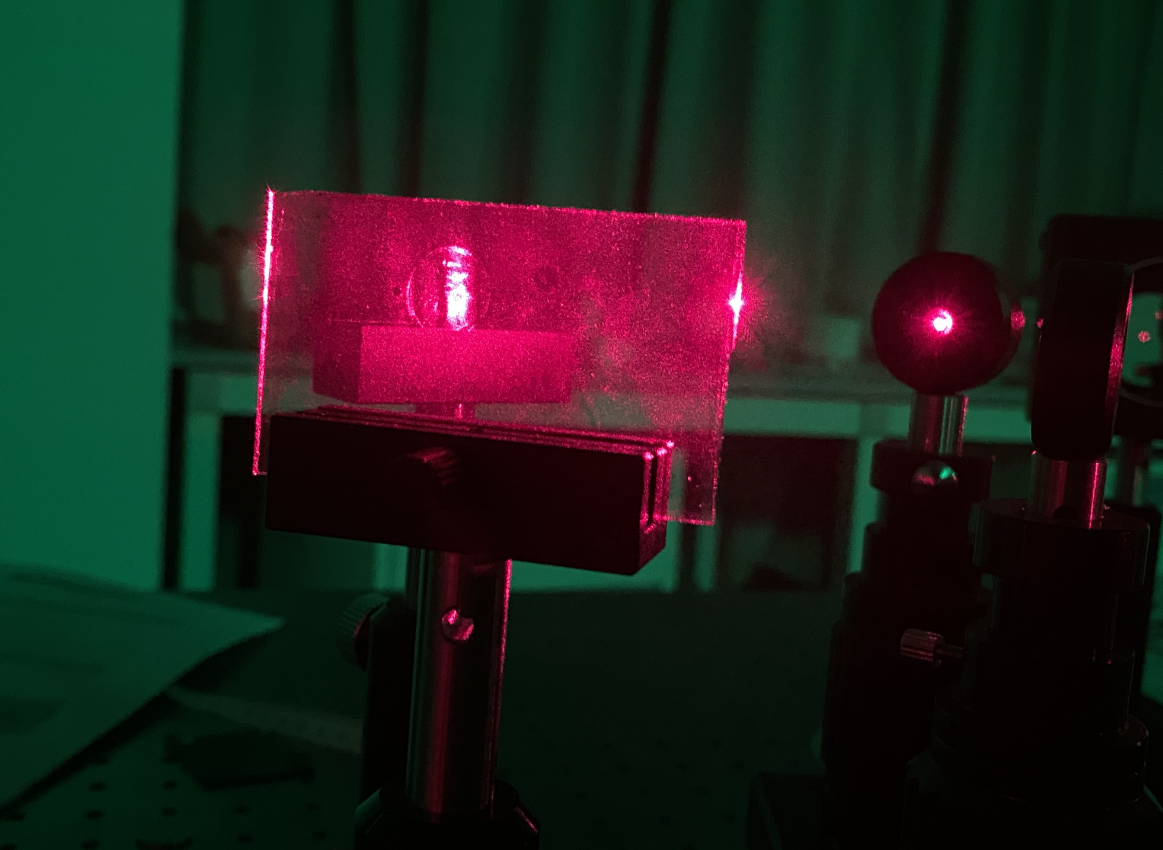
\includegraphics[clip,scale=0.8,trim={0 0 0 0}]{fig/fig7.png}
           	        \caption{image of a ten cent coin }
           	        \label{figure.14}
               \end{figure}

       	\begin{figure}[H]
           	    	\centering
           	    	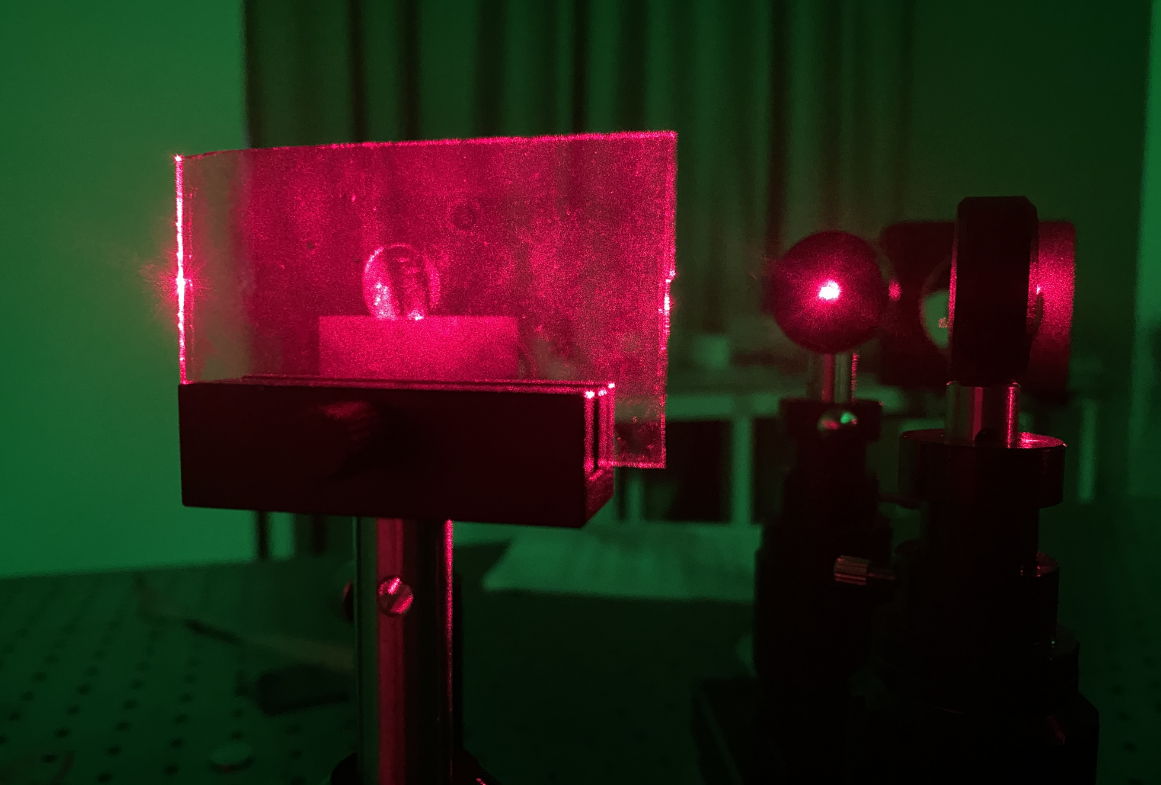
\includegraphics[clip,scale=0.8,trim={0 0 0 0}]{fig/fig8.png}
           	        \caption{image of a ten cent coin }
           	        \label{figure.14}
               \end{figure}
               
\subsection{Error analysis}
\begin{itemize}
  \item **Exposure Time Selection:** The chosen exposure time is critical in holography, as it affects the quality of the hologram. Errors in exposure time can lead to underexposed or overexposed holograms, resulting in reduced image clarity and contrast.

  \item **Alignment and Centering:** Accurate alignment and centering of optical components are essential. Errors in the alignment can cause shifts in the reconstructed images, affecting their accuracy and stability.

  \item **Vibration and Stability:** Vibrations or instability in the experimental setup can introduce errors. Even slight movements can lead to interference fringe displacement and distortions in the hologram.

  \item **Angular Alignment:** The angle (θ) between the object and reference beams must be within the specified range (30° to 45°). Deviations from this range can affect fringe spacing and result in poor interference patterns.

  \item **Developing and Fixing Times:** Errors in the developing and fixing times can impact the hologram's quality. Insufficient or excessive time in these steps can lead to inadequate fixing or over-processing, affecting the final image.

  \item **Observation Angle:** The angle at which the hologram is observed can influence the visibility of virtual and real images. Errors in selecting the observation angle may lead to difficulties in image observation.
\end{itemize}


\begin{appendix}
\section{Experimental procedure diagram}
	\begin{figure}[H]
           	    	\centering
           	    	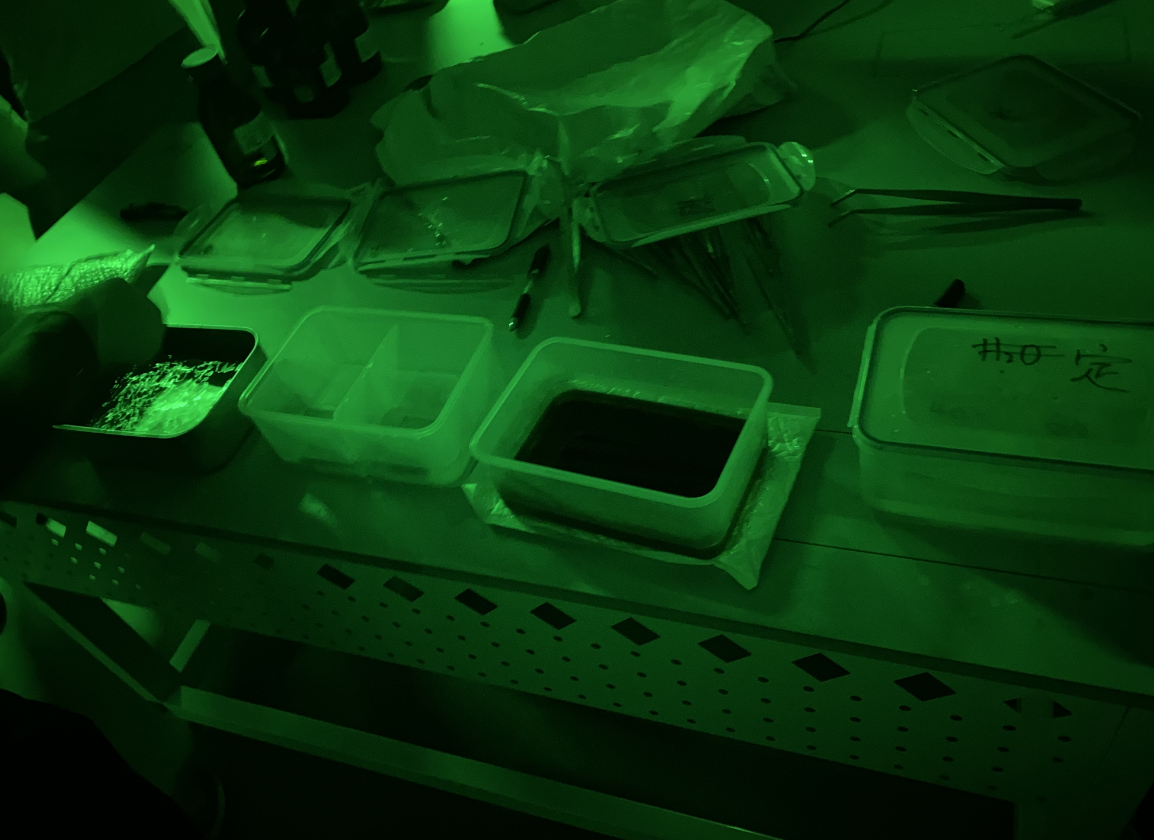
\includegraphics[clip,scale=0.75,trim={0 0 0 0}]{fig/fig9.png}
           	        \label{figure.14}
               \end{figure}

       	\begin{figure}[H]
           	    	\centering
           	    	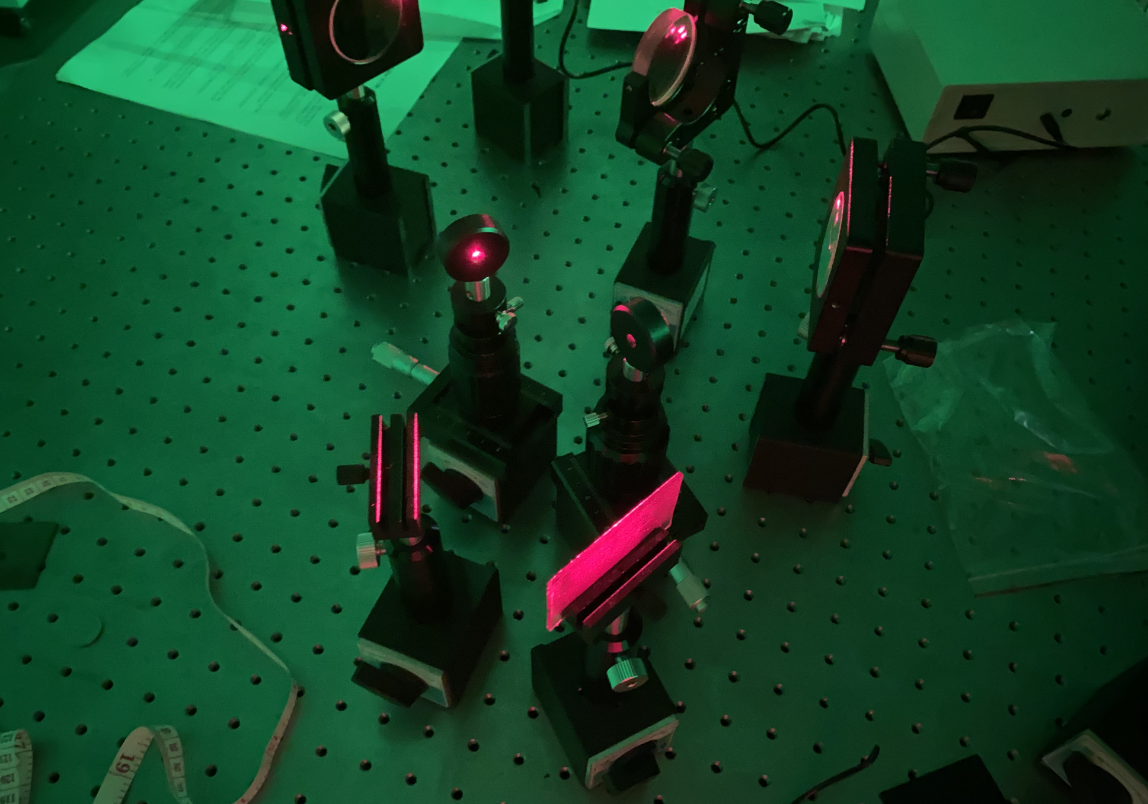
\includegraphics[clip,scale=0.75,trim={0 0 0 0}]{fig/fig10.png}
           	        \label{figure.14}
               \end{figure}
 \end{appendix}        
\end{document}  